%!TEX root = main.tex

\section{Background}
Breast cancer is the number one most common cancer amongst women in Singapore. Early and accurate diagnosis of breast cancer is important for breast-saving and life-saving treatment. \\

The gold standard for the diagnosis of breast cancer is by surgically removing the breast lump with a complete microscopic examination of the breast tissue to look for cancer cells. \\

Fine needle aspiration is an alternative that allows the doctor to take out a small amount of tissue from the breast lump, without the need for surgery to remove the entire breast lump. By examining the characteristics of the cells, doctors have been able to diagnose breast cancer with variable success. Increasing the success of fine needle aspiration allows for diagnosis of breast cancer without the need for a woman to undergo surgery to remove the breast lump. \\

To resolve this, this project uses a fuzzy decision tree to classify breast tumor cells into malignant cancer cells or benign non-cancerous cells. \\

\section{Dataset}
The dataset used was the Breast Cancer Wisconsin (Diagnostic) Data Set from the University of Irvine (UCI) Machine Learning Repository.  

The dataset contained 569 instances, with no missing data. 357 instances were benign (not cancerous) and 212 were malignant (cancerous). \\

The features were computed from digitalized images of fine needle aspirates of breast tumors.  \\

The features describe 10 characteristics of the cell nuclei present in the images:

\begin{itemize}
	\item The radius of an individual nucleus
	\item The nuclear perimeter
	\item The nuclear area
	\item Compactness of the nucleus
	\item The smoothness of the contour of the nucleus
	\item The number of contour concavities
	\item The symmetry of the nuclear contour
	\item The texture of the cell nucleus
\end{itemize}

\begin{figure}
	\centering
	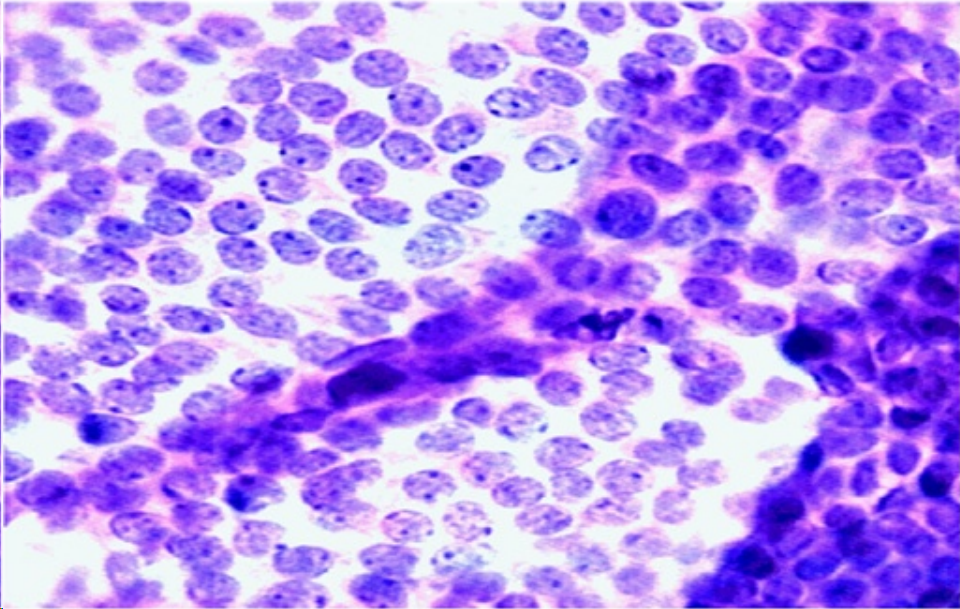
\includegraphics[width=0.45\linewidth]{screenshot001}
	\hspace{0.5cm}
	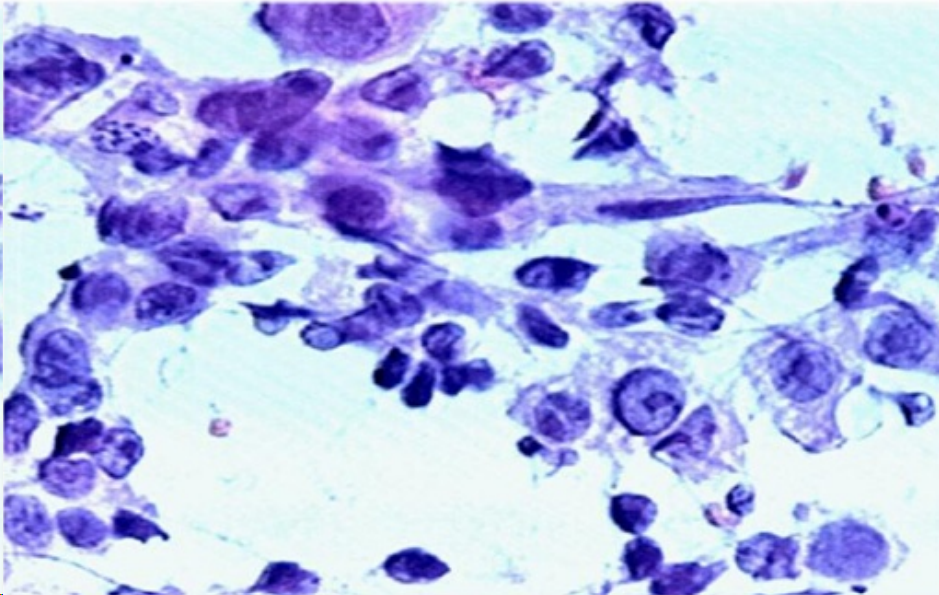
\includegraphics[width=0.45\linewidth]{screenshot002}
	\caption{A picture of breast cells. The cells on the left are begin while the cells on the right are cancerous.}
	\label{fig:images}
\end{figure}

The mean, standard error and worst (mean of the three largest values) of these features are computed for each image, resulting in 30 features in the UCI dataset. \\

\iffalse
We follow in the footsteps of Sizilio et al. \ref{fna} and add newly generated features of homogeneity and uniformity that were demonstrated to have diagnostic importance. \\

Uniformity is the difference between the radius worst value and the radius mean value and is an indication of the variability in size of the cell nuclei. \\

Homogeneity is the difference between the worst value of symmetry and the mean value of symmetry and is an indication of the symmetry of the cell nuclei. \\

According to Sizilio et al., the features of area, perimeter, homogeneity and uniformity produced the best results. Thus, we use these 4 feature and drop all other features. \\

The minimum and maximum area, perimeter, homogeneity and uniformity for the 2 labels (benign and malignant) are computed and displayed in the table below. \\

Fuzzy intervals are present for each of the above 4 features, whereby the benign values are within the range of the malignant values. This means that it is not linearly possible to diagnosis a breast lump as benign or malignant using a simple decision tree. Thus, we shall resort to using a fuzzy decision tree. \\

\section{Fuzzy Decision Tree}
A typical decision tree works by building a set of if statements to determine which class something belongs to. \\

At each branch of the decision tree, depending on whether a given statement is true / false, either the left or right path is chosen. \\

On the other hand, a fuzzy decision tree makes use of fuzzy logic, where the truth value of variables can range between 0 and 1 instead of being exactly 0 or exactly 1. \\
\fi

\section{Decision Tree}
To solve this problem, we will make use of a decision tree. In particular, we will use the Iterative Dichotomiser 3 (ID3) algorithm. \\

\heading{Entropy} A decision tree essentially asks certain questions at the right times, in order to determine which class the input belongs to. To do this, a value known as the entropy with the following formula is used.

$$E = \sum_{i=1}^{C}p_i\log_2 p_i$$

It measures the "impurity" of a set of objects. When the set is homogeneous (i.e. all the objects are of the same class), the entropy will be low. When the set is heterogeneous (i.e. the objects are from different classes), the entropy will be high. \\

\heading{Information Gain} In order to decide what question to ask at which point in time, we need to determine which question results in the greatest decrease in entropy. This is calculated using the information gain shown below:

$$IG = 1 - E$$

The feature that results in the greatest information gain will be selected for that branch of the tree. For continuous features, a threshold will be chosen based on what threshold will result in the greatest information gain. \\

Finally, we need to explain when the decision tree will decide when it should stop splitting. It will do this when the set is sufficiently pure (i.e. the entropy $E < E_C$ where $E_C$ is some critical value of entropy) or when a maximum depth $d_{max}$ has been reached. \\

\heading{Pseudocode} With this, we can now construct our decision tree. The pseudocode for construction and inference can be found below. 

\begin{itemize}
	\item \textbf{S} is the training data with $m$ classes and $n$ discrete features. It is defined as $\{\textbf{S} : \textbf{S} = {((f_1,f_2,\dots,f_n),c),f_i\in[1,\sf{len}(f_i)],c\in [1,m]}\}$\\
	\item $\sf{len}(f_i)$ refers to the number of values that the discrete feature can take on.\\
	\item We also define the node object $\textbf{N}$. It has a children attribute $N.\sf{children}$ which is a list of $\eta$ child nodes $\{\textbf{N}_1,\dots,\textbf{N}_\eta\}$. Furthermore, it also stores a function $func((f_1,f_2,\dots,f_n))$ which takes in a list of features and outputs an integer $i\in[1,\eta]$.
	
\end{itemize}

\begin{figure}[h]
	\oneCol{.9}{
		\alg{$\sf{BuildTree}(\bf{S}, d)$}
		Initialise new node $\textbf{N}$\\
		Initialise empty stack $\bf{L}$\\
		$\textbf{L}.\sf{push}((\textbf{S},\textbf{N}))$\\
		While $\textbf{L}.\sf{size}\neq0$ do\\
		\ind $\textbf{S}, \textbf{N}\gets \textbf{L}.\sf{pop}()$ \\
		\ind If $\textbf{N}.\sf{depth} > d$ then break \\
		\ind $E_{min}\gets\infty$ \\
		\ind For $i\in1\dots n$ do \\
		\ind \ind $E\gets 0$ \\
		\ind \ind For $j\in1\dots\sf{len}(f_i)$ do \\
		\ind \ind \ind $\textbf{S}_{new}\gets\{((f_1,f_2,\dots,f_n),c) : f_i=j, ((f_1,f_2,\dots,f_n),c)\in \textbf{S}\}$ \\
		\ind \ind \ind Calculate entropy $E'$ from $\textbf{S}_{new}$ \\
		\ind \ind \ind $E\gets E+E'$ \\
		\ind \ind If $E_{min} > E$ then \\
		\ind \ind \ind $E_{min}\gets E$ \\
		\ind \ind \ind $i_{min}\gets i$ \\
		\ind \ind \ind $\textbf{S}_{min}\gets \textbf{S}_{new}$ \\
		\ind \ind \color{gray}{End if} \\
		\ind \color{gray}{End for} \\
		\color{black}
		\ind For $j\in1\dots\sf{len}(f_i)$ do \\
		\ind \ind Initialise new node \textbf{M} \\
		\ind \ind $\textbf{N}.\sf{children}[i_{min}]\gets \textbf{M}$ \\
		\ind \ind $\textbf{L}.\sf{push}((\textbf{S}_{min},\textbf{M}))$\\
		\ind \color{gray}{End for} \\
		\color{gray}{End while}\\
		\color{black}Return $\textbf{N}$\\ \\
		\alg{$\sf{Qry({f_1,\dots,f_n},\textbf{N})}$}
		
	}
	\vspace{-.5cm}
	\caption{Pseudocode for construction and inference of the tree.}
	\label{fig-rh}
	\vspace{-.5cm}
\end{figure}

\section{Random Forest}
To improve the performance of our classifier, we make use of many different decision tree classifiers in an ensemble. \\
